\documentclass[border=4pt]{standalone}
\usepackage[compat=1.1.0]{tikz-feynman}
\tikzfeynmanset{every vertex={dot}}
\begin{document}
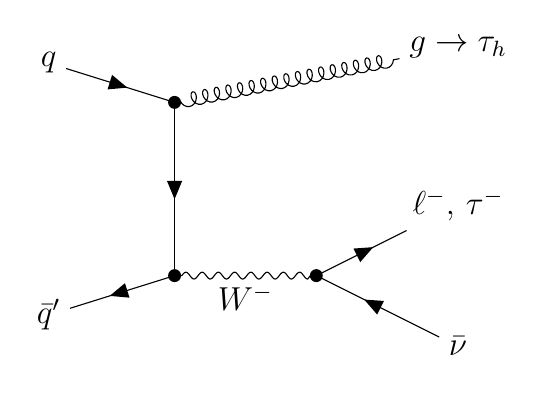
\begin{tikzpicture}[font=\large]
\begin{feynman}
\vertex (q) at (0, 1.6) {\(q\)};
\vertex (qb) at (0,-1.6) {\(\bar{q}'\)};
\vertex [dot] (v1) at (1.6, 1.1) {};
\vertex [dot] (v2) at (1.6,-1.1) {};
\vertex (j) at (5.2, 1.8) {\(g \to \tau_h\)};
\vertex [dot] (vw) at (3.4,-1.1) {};
\vertex (l) at (5.2,-0.2) {\(\ell^{-},\,\tau^{-}\)};
\vertex (n) at (5.2,-2.0) {\(\bar{\nu}\)};
\diagram*{
 (q) -- [fermion] (v1) -- [fermion] (v2) -- [fermion] (qb),
 (v1) -- [gluon] (j),
 (v2) -- [boson, edge label'=\(W^{-}\)] (vw),
 (vw) -- [fermion] (l),
 (vw) -- [anti fermion] (n),
};
\end{feynman}
\end{tikzpicture}
\end{document}
